% G07 - ECOM060 - Fase 2, Entrega 04: malha fechada com instrumentacao real
% Compilar com: xelatex relatorio.tex (duas vezes)
\documentclass[10pt,a4paper]{article}
\usepackage[margin=1.6cm,top=1.4cm,bottom=1.6cm]{geometry}
\usepackage{fontspec}
\setmainfont{TeX Gyre Termes}
\usepackage{amsmath,amssymb}
\usepackage{graphicx,booktabs,tabularx,multirow,array,xcolor}
\usepackage[font=small,labelfont=bf,labelsep=period]{caption}
\usepackage{enumitem}
\usepackage{newunicodechar}
\usepackage{placeins}
\newunicodechar{Ω}{\ensuremath{\Omega}}
\newunicodechar{→}{\ensuremath{\to}}
\newunicodechar{×}{\ensuremath{\times}}
\newunicodechar{·}{\ensuremath{\cdot}}
\newunicodechar{≤}{\ensuremath{\le}}
\newunicodechar{≈}{\ensuremath{\approx}}
\newunicodechar{°}{\ensuremath{^\circ}}
\newunicodechar{µ}{\ensuremath{\mu}}
\newunicodechar{Δ}{\ensuremath{\Delta}}
\usepackage[hidelinks]{hyperref}
\renewcommand{\figurename}{Figura}
\renewcommand{\tablename}{Tabela}
\renewcommand{\refname}{Referências}
\setlist{nosep,leftmargin=*}
\setlength{\parskip}{2pt}
\newcolumntype{Y}{>{\raggedright\arraybackslash}X}
\makeatletter\let\inputtab\@@input\makeatother
\newcommand{\R}[1]{\FloatBarrier\par\medskip\noindent{\large\bfseries #1}\par\smallskip}
\emergencystretch=3em\sloppy
\begin{document}
\begin{center}
{\Large\bfseries Malha fechada com instrumentação real: controle de corrente do motor BLDC MOONS' R42BLD30L3}\\[2pt]
Grupo G07 — Fase 2, Entrega 04 — ECOM060 Instrumentação Eletrônica (UFAL, 2026.2)\\[4pt]
\begin{tabular}{ll}\toprule Nome completo & Matrícula\\\midrule
Nícolas De Almeida Souza & 23111883\\ Lucas Momesso Alves & 22112804\\ Cláudio Henrique da Costa Santos & 20211850\\\bottomrule\end{tabular}
\end{center}

\R{Ponto de partida}
A planta é o equivalente elétrico da E02 \cite{e02}, executado no Virtual HIL (HIL101) e lido pelo HIL SCADA. A grandeza instrumentada na E03 \cite{e03} é a corrente de fase, medida pelo sensor Hall ACS712-20A com a cadeia real (sensibilidade, zero, banda, ruído, filtro RC de 15 kHz, ADC de 12 bits a 20 kS/s síncrono, correção calculada e média por período de PWM). A malha fechada sobre essa grandeza é a \textbf{malha de corrente}, que no motor equivale a uma malha de torque ($T_e = k\,i$). O que foi corrigido ao reaproveitar:
\begin{itemize}
\item \textbf{Segundo sensor, na fase b}, com a mesma cadeia e outro gerador de ruído. Com um sensor só, a corrente do par em condução não é conhecida em 2 de cada 6 setores. $i_c = -(i_a+i_b)$, como nos acionamentos comerciais.
\item \textbf{Grandeza controlada}: o módulo da corrente do par em condução, $i = (|i_a|+|i_b|+|i_c|)/2$, que vale a corrente da fonte no six-step e dispensa a posição. A mesma expressão sobre as correntes verdadeiras dá a \emph{grandeza real da planta}.
\item \textbf{Correção calculada com o zero calibrado.} Na E03 o processamento usava o próprio desvio de zero do sensor, o que equivale a uma calibração perfeita. Agora ele usa o valor calibrado (10 mV, caixa \texttt{G07\_V\_zero}), e o R4 varia o zero efetivo, o que representa deriva ou envelhecimento depois da calibração.
\end{itemize}
O controlador usa só blocos nativos (\texttt{Sum} e \texttt{PID controller} em modo PI, com anti-windup e limite 0–1). Ficam em \texttt{C function}, com justificativa: o cálculo de $|i_a|+|i_b|+|i_c|$ com troca ideal/real (a biblioteca não tem seletor de fonte de realimentação ajustável pelo SCADA), a geração da referência e das perturbações dos ensaios, e o modo 5 do seletor de razão cíclica herdado da E01.

\R{R1. Especificação de desempenho}
O motor aciona um ventilador (E01): a malha de corrente é a malha interna de um controle de velocidade e define o torque entregue. Os critérios vêm dessa aplicação e dos números das entregas anteriores (Tab.~\ref{tab:spec}). As métricas usam a média de dois intervalos de comutação (120° elétricos, ≈1,3 ms), porque a corrente do par em condução tem uma ondulação física de cerca de $\pm$0,3 A a cada comutação (Fig.~\ref{fig:r3}): é o valor médio que produz torque.

\begin{table}[!htbp]\centering\footnotesize
\caption{Critérios de desempenho da malha de corrente (referência de 1,5 A, próxima da corrente de 1,675 A do equilíbrio de 4000 rpm da E01).}\label{tab:spec}
\begin{tabularx}{\textwidth}{p{3.2cm}p{2.6cm}Y}\toprule
Critério & Valor & Justificativa\\\midrule
Erro estacionário & $|e_{ss}| \le$ 30 mA (2 \%) & erro de torque de 2 \%; o mesmo limite de viés da E03\\
Tempo de acomodação ($\pm$5 \%) & $\le$ 3 ms & a malha de velocidade da E01 acomoda em ≈11 ms; a malha interna deve ser pelo menos 3 a 4 vezes mais rápida\\
Sobressinal & $\le$ 10 \% & sobrecorrente e pico de torque no ventilador\\
Esforço de controle & desvio-padrão de $d \le$ 0,08; saturação $\le$ 1 \% do tempo & ±0,08 em $d$ = ±2,9 V de ruído na tensão aplicada; saturar significa perder o controle\\
Rejeição de perturbação & $|\Delta i| \le$ 0,30 A (20 \%), volta à faixa de 5 \% em $\le$ 5 ms & perturbação: afundamento de 10 \% da tensão (Δ$d$ = $-$0,1 ≈ 3,6 V) e pulso de carga de 0,02 N·m (terceiro ensaio da E01)\\\bottomrule
\end{tabularx}
\end{table}

\R{R2. Controlador com instrumentação ideal}
\textbf{Modelo e método de sintonia.} Com duas fases em série, a planta vista da razão cíclica é $G(s) = \dfrac{V_s}{L_{LL}s + R_{LL}}$, com $V_s$ = 36 V, $L_{LL}$ = 3,8 mH e $R_{LL}$ = 3,2 $\Omega$ (E01). A FCEM entra como perturbação lenta. Sintonia por \textbf{cancelamento de polo}: o zero do PI, $K_i/K_p = R_{LL}/L_{LL}$ = 842 s$^{-1}$, cancela o polo elétrico, e a malha fica $L(s) = \frac{\omega_c}{s}e^{-s\tau}$, com $\omega_c = K_pV_s/L_{LL}$. Escolhemos $\omega_c$ = 2500 rad/s, o que dá $K_p$ = 0,264 e $K_i$ = 222 s$^{-1}$. O atraso $\tau$ vale meio período de PWM (50 µs) com a medição ideal e 110 µs com a real (mais os 60 µs medidos na E03).

\textbf{Previsão algébrica.} Polo de malha fechada em $s = -\omega_c$ = $-$2500 rad/s (constante de tempo de 0,40 ms), sem sobressinal, com $t_s(\pm5\,\%) = \ln 20/\omega_c$ = 1,2 ms. Margem de fase $90° - \omega_c\tau$ = 83° (ideal) e 74° (real). Margem de ganho $\pi/(2\omega_c\tau)$ = 12,6 (22 dB) e 5,7 (15 dB) (Fig.~\ref{fig:bode}). Erro estacionário nulo ao degrau de referência e ao degrau de perturbação na entrada (tipo 1). A FCEM em rampa durante a aceleração deixa um erro de $\dot E/(V_s K_i)$ ≈ 20 mA. O afundamento de Δ$d$ = $-$0,1 dá $\Delta i(t) = \frac{\Delta d\,V_s}{L_{LL}(\omega_c - a)}(e^{-at} - e^{-\omega_c t})$, com $a = R_{LL}/L_{LL}$: pico de $-$0,22 A em 0,66 ms e volta à faixa de 5 \% em 2,4 ms.

\begin{figure}[!htbp]\centering
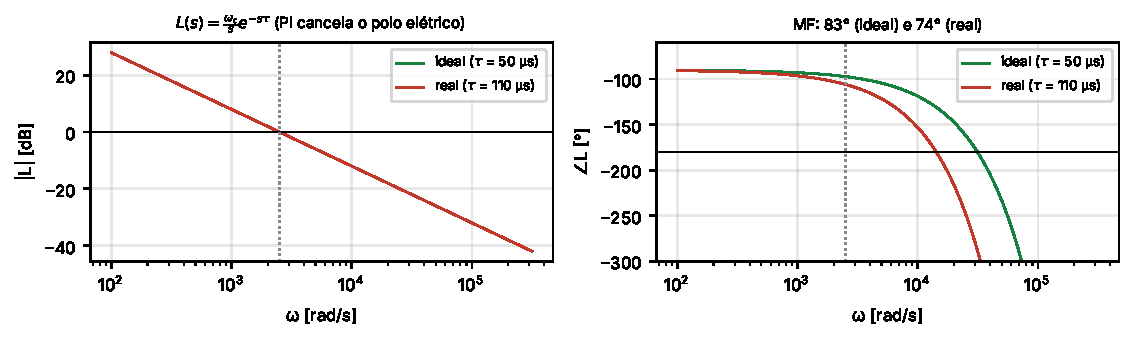
\includegraphics[width=\textwidth]{figuras/fig_bode.pdf}
\caption{Ganho de malha previsto, com os atrasos da medição ideal e da real.}\label{fig:bode}
\end{figure}

\textbf{Verificação.} Com a medição ideal (Tab.~\ref{tab:r3}, coluna "ideal"), a corrente sobe para a nova referência em menos de 1 ms, acomoda em 1,4 ms (previsto: 1,2 ms), tem 5 \% de sobressinal e 9 mA de erro estacionário. O erro de 9 mA é o efeito previsto da FCEM em rampa, que aparece como uma subida lenta nos 10 ms seguintes ao degrau, enquanto o motor acelera. O afundamento dá $-$0,17 A, contra $-$0,22 A previstos; a média de 1,3 ms suaviza o pico. A recuperação leva 2,1 ms (previsto: 2,4 ms). Todos os critérios do R1 são atendidos.

\R{R3. Mesma malha com instrumentação real}
\begin{figure}[!htbp]\centering
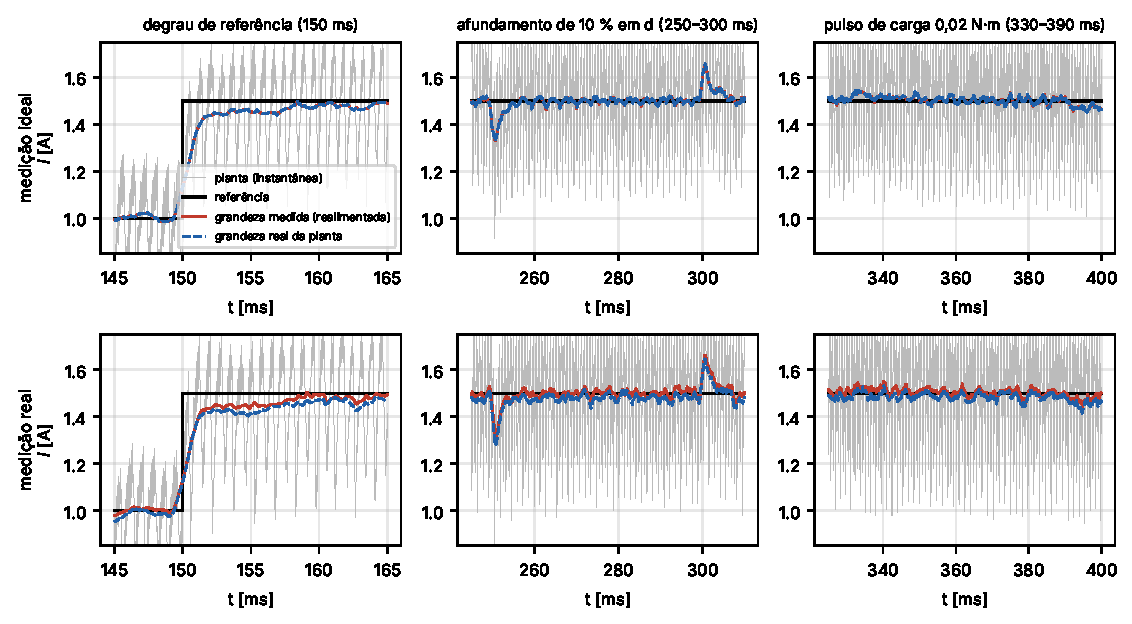
\includegraphics[width=\textwidth]{figuras/fig_r3.pdf}
\caption{Os três ensaios, com a medição ideal (em cima) e a real (embaixo) realimentando o mesmo PI: referência, grandeza medida (realimentada), grandeza real da planta (média de 2 intervalos de comutação) e a planta instantânea (cinza).}\label{fig:r3}
\end{figure}

\begin{table}[!htbp]\centering\footnotesize
\caption{Métricas do R1 com a medição ideal, e com a real (grandeza medida e grandeza real da planta). $\times$ = critério não atendido.}\label{tab:r3}
\begin{tabular}{lrrrr}\toprule
Critério & Limite & Ideal & Real: medida & Real: planta\\\midrule
\inputtab tabelas/tab_r3.tex \bottomrule
\end{tabular}
\end{table}

\textbf{Explicação das diferenças.} (i) \emph{Erro estacionário}: o PI zera o erro \emph{da medida} (5 mA), mas a planta fica 23 mA abaixo. A causa é o \textbf{ruído retificado}: no setor em que uma fase não conduz, sua corrente é nula e a medida é só ruído; $|n|$ tem média $\sigma\sqrt{2/\pi}$, que soma um viés positivo. Com o ruído na saída da cadeia ($\sigma \approx$ 34 mA, E03), a média sobre os seis setores dá $0{,}455\sigma \approx$ 16 mA. Com a malha ideal, a medida real (não realimentada) fica 20 mA acima da planta. Ainda está dentro dos 30 mA. (ii) \emph{Atraso}: os 60 µs da média por período e da amostragem reduzem a margem de fase de 83° para 74° e elevam o sobressinal de 5 para 6–7 \%. (iii) \emph{Acomodação da planta}: 4,8 ms com a faixa de 5 \% contra 1,3 ms na medida. É o mesmo transitório (com faixa de 10 \%, 0,8 ms nos três casos): a planta acomoda 23 mA abaixo, perto da borda da faixa, e um pico da ondulação de comutação sai dela; é um efeito do viés (i), não de lentidão. (iv) \emph{Perturbações}: $|\Delta i|$ de 0,20 A contra 0,17 A, por causa do mesmo atraso; o pulso de carga quase não aparece na corrente (0,04 A), porque age na velocidade e chega à malha de corrente como uma variação lenta da FCEM. (v) \emph{Esforço}: praticamente igual (0,049 contra 0,047). A média por período retira da realimentação a ondulação de 10 kHz, e o ruído restante, multiplicado por $K_p$ = 0,26, dá só 0,009 em $d$.

\R{R4. Intensidade das características em malha fechada}
Foram varridas três características do R5 da E03, cada uma em quatro níveis, num único ensaio de 0,5 s: o próprio modelo troca o nível a cada 0,1 s (\texttt{g07\_cl\_ens} = 2, 3 e 4). Em cada nível há um degrau de 1,0 para 1,5 A e um afundamento de 10 \%. As previsões foram feitas antes de simular:
\begin{itemize}
\item \textbf{Desvio de zero não compensado} $\delta$ = $e_Q/S$ por fase (a fase c herda $-2\delta$). No setor em que a fase não conduz, a medida soma $|\delta|$; a média sobre os setores dá $\frac{2}{3}|\delta|$, então a planta fica em $i^* - \frac23\delta$. A malha colapsa quando a medida com corrente nula, $2\delta$, passa de $i^*$, ou seja $\delta >$ 0,75 A (75 mV).
\item \textbf{Filtro RC}: as correntes de fase são alternadas, com $f_e \approx$ 247 Hz a 3700 rpm. O filtro atenua a amplitude por $|H(f_e)| = 1/\sqrt{1+(f_e/f_c)^2}$, e a planta sobe para $i^*/|H|$. O atraso de grupo $\approx 1/(2\pi f_c)/(1+(f_e/f_c)^2)$ reduz a margem de fase.
\item \textbf{Ruído}: viés de $0{,}455\,\sigma_f$, com $\sigma_f = \sigma_v\sqrt{\frac{\pi}{2}\frac{15}{100}}/(\sqrt2\,S)$ depois do RC e da média; o esforço sobe com $K_p\sigma_f$.
\end{itemize}

\begin{figure}[!htbp]\centering
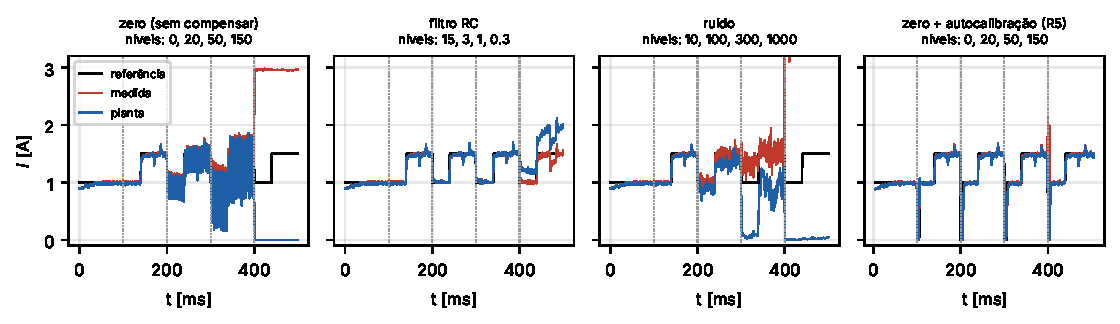
\includegraphics[width=\textwidth]{figuras/fig_varreduras.pdf}
\caption{Varreduras no VHIL (níveis trocados a cada 0,1 s, linhas pontilhadas): referência, grandeza medida e grandeza real da planta. À direita, o mesmo zero com a ação do R5.}\label{fig:var}
\end{figure}

\begin{table}[!htbp]\centering\footnotesize
\caption{Previsão e resultado por nível (erro = referência $-$ planta; $\times$ = critério do R1 não atendido). O nível nominal da E03 é o primeiro de cada bloco.}\label{tab:r4}
\begin{tabular}{llrrrrrr}\toprule
Característica & Nível & Erro previsto [mA] & Erro [mA] & Sobressinal [\%] & Desvio de $d$ & Saturado [\%] & $|\Delta i|$ [A]\\\midrule
\inputtab tabelas/tab_r4.tex \bottomrule
\end{tabular}
\end{table}

\begin{figure}[!htbp]\centering
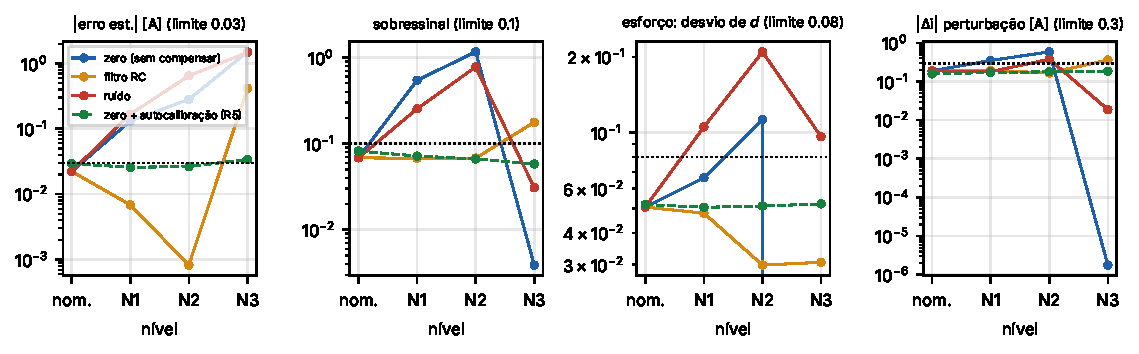
\includegraphics[width=\textwidth]{figuras/fig_mapa.pdf}
\caption{Mapa de desempenho: cada critério do R1 (linha pontilhada = limite) em função do nível de cada característica.}\label{fig:mapa}
\end{figure}

\textbf{A partir de onde cada critério falha} (interpolação entre os níveis da Tab.~\ref{tab:r4}):
\begin{itemize}
\item \textbf{Desvio de zero não compensado.} O erro estacionário falha já com \textbf{1,4 mV}. A previsão é de 1,2 mV, considerando que o ruído já consome 22 dos 30 mA: $\frac23\delta \le$ 8 mA. O sobressinal falha com 1,3 mV, o esforço com 29 mV e a rejeição com 14 mV. Com 150 mV a malha colapsa: a medida marca 3 A com a corrente nula, e a razão cíclica vai a zero, como previsto.
\item \textbf{Filtro RC.} Em 3 e 1 kHz o efeito é pequeno, e a atenuação até compensa parte do viés do ruído. Em 0,3 kHz a planta vai a 1,91 A (previsto: 1,94 A), e falham o erro, o sobressinal e a rejeição. Os limites ficam em $f_c \approx$ 0,95 kHz para o erro (previsto: 1,2 kHz), 0,8 kHz para o sobressinal e 0,5 kHz para a rejeição. O esforço não chega a falhar: o filtro também tira ruído da realimentação.
\item \textbf{Ruído.} O erro falha com \textbf{15 mV} (previsto: 19 mV), o sobressinal com 25 mV, o esforço com 58 mV (previsão por $K_p\sigma_f$: 74 mV) e a rejeição com 220 mV; com 300 mV a razão cíclica já satura 3 \% do tempo. Com 300 mV a planta cai para 0,89 A. Com 1 V a medida passa de 4 A com a corrente quase nula, e a malha satura em zero.
\end{itemize}
O tempo de acomodação não entra no mapa: em cada nível o motor ainda está acelerando, e a métrica fica dominada pela rampa da FCEM. Seu efeito aparece no sobressinal, que usa o mesmo degrau. A medição real nominal da E03 atende a todos os critérios, mas com pouca folga no erro estacionário (22 de 30 mA), justamente por causa do ruído retificado.

\R{R5. Ação de projeto: autocalibração do zero}
O R4 mostrou que o critério mais frágil é o erro estacionário, e que o zero não compensado o derruba com só 1,4 mV, menos que a deriva térmica de 60 °C a 25 °C (2,5 mV, E03). A melhoria é no \textbf{processamento}: uma \textbf{autocalibração do zero} (caixa \texttt{G07\_autocal}). Ao ligar, e a cada nível na varredura, o controle zera a razão cíclica por 5 ms. A corrente cai a zero, porque com $d$ = 0 os diodos bloqueiam, como no ensaio (b) da E01. Depois de 3 ms o processamento média as amostras do ADC e passa a usar esse valor como zero. É a correção calculada da Seção 2.5.3 de Aguirre \cite{aguirre}: a entrada interferente (o zero) é medida numa condição conhecida ($i = 0$) e descontada.

\textbf{Resultado} (Tab.~\ref{tab:r4}, último bloco; Fig.~\ref{fig:var}, à direita): o erro estacionário fica entre 26 e 29 mA com o zero não compensado de 0 a 50 mV, contra 22, 132 e 282 mA sem a ação. O limite para o erro sobe de 1,4 mV para 97 mV, e os demais critérios passam em todos os níveis. Com 150 mV ficam 34 mA, porque o ruído retificado continua (a autocalibração não o remove).

\textbf{Custo.} (i) \emph{Complexidade}: uma sequência de partida e uma média no processamento (cerca de 15 linhas em C), sem hardware novo. (ii) \emph{Atraso}: nenhum dentro da malha. O custo é uma interrupção de torque de 5 ms em cada calibração; só na partida, isso é imperceptível no ventilador, e se for repetida para acompanhar a deriva térmica, cada repetição é um "buraco" de torque. (iii) \emph{Esforço}: o mesmo (0,051 a 0,052). As alternativas do Cap.~2 têm outros custos: insensibilidade inerente (sensor Hall em malha fechada de fluxo, ou seja realimentação, 2.5.5) exige outro componente; entradas opostas (2.5.4: medir as três fases e impor $i_a+i_b+i_c$ = 0 para estimar o zero) exige um terceiro sensor. Para o viés do ruído retificado, a ação seria trocar $|i_a|+|i_b|+|i_c|$ pela seleção da fase em condução pelos sensores Hall de posição, que eliminaria a fase só com ruído. Fica como próxima melhoria.

\R{R6. Síntese e repetibilidade}
\textbf{Síntese.} Em malha fechada, o controlador zera o erro \emph{da medida}: tudo o que desloca a média da medida aparece inteiro, com sinal trocado, na grandeza real. No nosso sistema, isso faz do \textbf{desvio de zero} a característica decisiva. Ele entra pela fase que não conduz, multiplicado por 2/3, e derruba o erro estacionário com 1,4 mV, menos que a deriva térmica do próprio sensor. Logo depois vem o \textbf{ruído}: em malha aberta (E03) ele só espalhava a medida, mas aqui a operação $|\cdot|$ o converte em viés, a partir de 15 mV. A banda (filtro RC) só pesa quando chega perto da frequência elétrica: abaixo de ≈1 kHz atenua as correntes alternadas e a planta passa da referência. Atraso, sobressinal e esforço estão folgados com os valores reais. Para a instrumentação, isso indica: (1) calibrar o zero com o inversor parado (R5), ou escolher um sensor de menor deriva; (2) manter o ruído baixo antes de retificar, ou usar a posição para escolher a fase em condução; (3) manter o filtro anti-aliasing acima de 4 vezes a frequência elétrica máxima.

\textbf{Roteiro.}
\begin{enumerate}
\item Typhoon HIL Control Center \textbf{2026.3}. Arquivos (pasta \texttt{entregas/fase-2/e4-malha-fechada/simulacao/}): \texttt{modelo\_malha\_fechada.tse} e \texttt{painel\_malha\_fechada.cus}.
\item Abrir o \texttt{.tse} no Schematic Editor, perspectiva \textbf{tempo real}. Em \emph{Model initialization}, colar o bloco da Tab.~\ref{tab:rot} (de \texttt{g07\_modo} a \texttt{g07\_cl\_ens}) e compilar. O console deve mostrar \texttt{G07 E04: malha de corrente Kp=0.2639 Ki=222.2}.
\item No HIL SCADA, carregar \texttt{modelo\_malha\_fechada Target files/modelo\_malha\_fechada.cpd} em \textbf{Virtual HIL} e abrir \texttt{painel\_malha\_fechada.cus}. Ajustar no painel \texttt{G07\_fb\_real} e \texttt{G07\_autocal} (Tab.~\ref{tab:rot}); as demais caixas ficam nos valores da E03. Após cada compilação, \emph{Model > Reload Model}.
\item No Capture, escolher o preset (\textbf{Default} = 0,45 s; \textbf{R4\_varredura} = 0,5 s; ambos a 100 kS/s, gatilho em \texttt{G07\_cl\_ref}). Com a simulação parada, clicar em \textbf{T↑} e depois em \emph{Start simulation}. Exportar em CSV para \texttt{dados-vhil-e4/}.
\item Demonstração ao vivo: com a sequência do R3 rodando, mudar \texttt{G07\_fb\_real} (0/1), \texttt{G07\_corr} = 0 (sem correção calculada: o zero de 7,5 mV deixa de ser descontado; previsão: a planta cai ≈ 65 mA), \texttt{G07\_ruido} = 100 (planta ≈ 1,32 A) ou \texttt{G07\_fc\_rc} = 0.3 (planta ≈ 1,9 A) e comparar \texttt{G07\_cl\_med} com \texttt{G07\_cl\_planta}. A caixa \texttt{G07\_V\_zero} muda o zero efetivo e o calibrado juntos, então não mostra o efeito do zero; ele aparece nas varreduras.
\end{enumerate}

\begin{table}[!htbp]\centering\footnotesize
\caption{Capturas e resultado esperado. Linhas comuns do bloco: \texttt{g07\_modo = 5}, \texttt{g07\_d0 = 0.7074}, \texttt{g07\_d\_ini = 0.0}, \texttt{g07\_d\_deg = 0.7074}, \texttt{g07\_t\_deg = 0.0}, \texttt{g07\_t\_ci = 0.15}, \texttt{g07\_d\_ci = 0.0}, \texttt{g07\_Td = 0.02}.}\label{tab:rot}
\begin{tabularx}{\textwidth}{p{2.6cm}p{3.6cm}p{2.3cm}p{2.0cm}Y}\toprule
Captura (CSV) & Bloco & Painel & Preset & Esperado\\\midrule
\texttt{e4\_r3\_ideal} & \texttt{g07\_t\_p1 = 0.33}, \texttt{g07\_t\_p2 = 0.39}, \texttt{g07\_cl\_ens = 1} & \texttt{fb\_real} = 0, \texttt{autocal} = 0 & Default & coluna "ideal" da Tab.~\ref{tab:r3}\\
\texttt{e4\_r3\_real} & idem & \texttt{fb\_real} = 1 & Default & planta ≈ 1,478 A com a referência de 1,5 A\\
\texttt{e4\_r4\_zero} & \texttt{g07\_t\_p1 = 1.0}, \texttt{g07\_t\_p2 = 1.1}, \texttt{g07\_cl\_ens = 2} & \texttt{fb\_real} = 1 & R4\_varredura & planta 1,48 / 1,38 / 1,22 / 0 A\\
\texttt{e4\_r4\_rc} & idem, \texttt{g07\_cl\_ens = 3} & \texttt{fb\_real} = 1 & R4\_varredura & 1,48 / 1,49 / 1,50 / 1,91 A\\
\texttt{e4\_r4\_ruido} & idem, \texttt{g07\_cl\_ens = 4} & \texttt{fb\_real} = 1 & R4\_varredura & 1,48 / 1,32 / 0,89 / 0,03 A\\
\texttt{e4\_r5\_autocal} & idem, \texttt{g07\_cl\_ens = 2} & \texttt{fb\_real} = 1, \texttt{autocal} = 1 & R4\_varredura & 1,47–1,48 A em todos os níveis\\\bottomrule
\end{tabularx}
\end{table}

\begin{thebibliography}{9}\small
\bibitem{aguirre} L. A. Aguirre. \emph{Fundamentos de Instrumentação}. São Paulo: Pearson, 2013 (Cap. 2, Seções 2.5.1 a 2.5.5).
\bibitem{e02} G07. Equivalente elétrico no TyphoonSim: motor BLDC MOONS' R42BLD30L3 (Fase 2, Entrega 02). ECOM060, UFAL, 2026.
\bibitem{e03} G07. Instrumentação em malha aberta: corrente de fase do motor BLDC (Fase 2, Entrega 03). ECOM060, UFAL, 2026.
\bibitem{acs712} Allegro MicroSystems. \emph{ACS712}, datasheet ACS712-DS.
\bibitem{ty} Typhoon HIL. Schematic Editor, HIL SCADA e Capture/Scope — documentação da versão 2026.3.
\end{thebibliography}

\appendix
\section*{Apêndice A. Código externo novo (\texttt{C function})}
O código completo está no \texttt{.tse} e em \texttt{simulacao/codigo\_c\_functions.md}. Os blocos da cadeia real são os da E03 (os da fase b são cópias com sufixo \texttt{\_b}).
\begin{table}[!htbp]\centering\footnotesize
\begin{tabularx}{\textwidth}{p{3.6cm}p{3.0cm}Y}\toprule
Bloco & Entradas → saídas & Operação\\\midrule
\texttt{G07\_CL\_referencia} & zero, RC e ruído do SCADA, \texttt{autocal} → $i^*$, Δ$d$, \texttt{cal}, zero, RC e ruído efetivos & gera a sequência do R3 (degrau, afundamento) ou a varredura do R4 (4 níveis de 0,1 s) e as janelas de calibração; com a varredura desligada, repassa os valores do SCADA\\
\texttt{G07\_CL\_realimentacao} & $i_a$, $i_b$ ideais e reais, \texttt{fb\_real} → $i_{fb}$, $i_{planta}$, $i_{medida}$ & $i = (|i_a|+|i_b|+|i_a+i_b|)/2$; escolhe a fonte realimentada\\
\texttt{G07\_P1\_processamento} (modificado) & + \texttt{cal}, \texttt{autocal} & na janela de calibração, média das amostras após 3 ms; depois usa a média como zero\\
\texttt{G07\_Seletor\_duty} (modificado) & + $d_c$, \texttt{cal} & modo 5: $d = d_c$ limitado a 0–1, e 0 durante a calibração\\\bottomrule
\end{tabularx}
\end{table}
\end{document}
